\chapter{Introduction}
\label{introduction}

% The confluence of advanced recording techniques for measuring neural 
% activity and scalable machine learning algorithms makes this a 
% particularly exciting time in computational neuroscience. In some organisms,
% we already have access to whole-brain recordings. In order to understand the 
% computations neural circuits implement, we need to approach this problem 
% from the both the top down and the bottom up. That is, we need 
% theories of neural computation that rest on principled foundations, and 
% we need statistical methods capable of instantiating these theories 
% in probabilistic models and testing them against large-scale brain recordings.
% This thesis is about building a suite of statistical models and computational 
% algorithms that expands the frontier of models that we can efficiently 
% instantiate and fit. In doing so, we continue to close the gap between our theory 
% of neural computation and our methods of analysis.

Neuroscience is undergoing a technological revolution. Where
traditional methods were limited to either direct measurements of a
handful of neurons or gross measurements of
%average activity in
entire brain volumes, modern calcium imaging techniques and
microelectrode arrays enable precise measurements of thousands of
neurons at a time. For some organisms, we can now monitor the activity
of every single neuron in the brain.
At the same time, advances in connectomics --- the
mapping of synaptic connectivity --- are providing a
more complete atlas of the wiring diagram that underlies neural
activity.  Likewise, sophisticated tracking and processing algorithms
are providing rich descriptions of the overt, natural behavior that
this activity gives rise to.  These unprecedented technological
capabilities are leading to a fundamental paradigm shift.
% Paradigm shift -> data-driven science
% new datasets contain patterns that can expose where existing theories fall short
% new data contains patterns that can suggest new hypotheses, model additions
Questions that were once intractable due to impoverished data,
questions about the structure and dynamics of neural computation,
can now be tackled with large-scale recordings.
%Questions about the structure and dynamics of neural computation, once
%intractable due to impoverished data, can now be tackled.
What we lack are complementary computational and statistical tools to
discover this hidden structure in neural data.  This thesis develops a
set of modeling tools and inference algorithms to address this
pressing need.

\section{Networks as Concise Representations of Complex Systems}
Networks play a central role in modern neuroscience: they distill
complex systems into concise representations.  The goal of
connectomics \cite{sporns2005human} is to build a wiring diagram, or
``connectome,'' of the brain. Each neuron in the brain is a node in
this network, and the edges correspond to individual connections
between from one neuron to another. These connections are called
\emph{synapses}, and they are how spikes on one neuron influence the
subsequent activity of another.  Once we have extracted this massive
network of synaptic connections, we can perform subsequent analyses,
searching for recurring patterns that will illuminate underlying
design principles and, hopefully, provide insight into neural
computation \cite{bullmore2009complex}.

%Building this wiring diagram, or ``connectome'', is a painfully
%tedious process that involves slicing sections of brain tissue
%nanometers thin, scanning them with an electron microscope, segmenting
%the resulting images to identify cell bodies and synapses, and then
%reconstructing the three dimensional volume of tissue
%\cite{white1986structure, lichtman2008technicolour,
%  helmstaedter2013connectomic, oh2014mesoscale} .  Needless to say,
%this process is both computationally demanding and prone to errors.

Networks need not be so fine grained, however.  Systems neuroscientists
often describe intricate circuits with simplified networks whose nodes
correspond to populations of cells, and whose edges denote the an
abundance connections from one population to another
\cite[e.g.]{felleman1991distributed, scannell1999connectional}.  Since
neurons in a particular brain region often have highly stereotyped
patterns of connectivity, it is convenient to describe neural circuits
in terms of block diagrams.  These abstract networks do not capture
the nuances of synaptic connections, but they do provide concise
representations of neural computation.

Even in functional magnetic resonance imaging (fMRI) studies, where the
recorded voxels correspond to hundreds of thousands of neurons, networks
are used to describe \emph{functional connectivity} between brain regions
\cite{friston1994functional}. While these networks are far removed from
the underlying synaptic connectivity, they exhibit telling differences
in healthy and diseased patients \cite{bassett2008hierarchical}
and show complex structure that is far from random \cite{bassett2006small}.

In fact, network models need not be derived from data at all.  Many
theoretical models of neural computation use networks to describe
idealized interactions between neurons. These interactions are only
loosely based on the known properties of neurons and
synapses. Nevertheless, these theoretical network models provide
invaluable insight into the properties of complex systems
\cite{hopfield1982neural, amit1992modeling, van1996chaos, DayanAbbott,
  sussillo2009generating}.



The goal of Chapters~\ref{chap:three},~\ref{chap:four},
and~\ref{chap:five} is to 


% Problem: translating neural activity into understanding
\section{Four Challenges in Deciphering Neural Computation}
The origins of human intelligence have puzzled scientists and
philosophers since the days of ancient Greece, and they remain largely
a mystery to this day. Through centuries of painstaking
experimentation, the brain and its network of neurons have been
identified as the seat of intelligence, and their physiology has been
carefully catalogued. The human brain has on the order
of~$\text{10}^{\text{10}}$ neurons, which are considered to be the
fundamental units of computation. Neurons are electrically excitable
cells with time-varying membrane potentials. When the membrane
potential is excited above a certain threshold, a cascade of ion
channels opens and closes, causing the membrane potential to undergo a
characteristic action potential, or ``spike.''

% Spike hypothesis: at the heart of this computation is the action potential,
% or ``spike.'' These spikes are 
These spikes encode information about the state of the outside world
as conveyed by our sensory organs. Moreover, they represent internal
states about plans, goals, desires, and thoughts. The spikes of our
motor neurons travel down our spinal cord, innervating our muscles and
giving rise to our overt behavior. To first approximation, spikes are
fundamentally discrete events in time.  That is, in a short enough
window of time, a neuron either does or does not fire an action
potential.  The first challenge of deciphering neural computation is
understanding how information about external and internal states is
encoded in discrete patterns of coordinated spiking activity across
neural circuits.

The second is understanding how this information is transformed over
time. The neurons in our brain are connected by
about~$\text{10}^{\text{14}}$ synapses. When a pre-synaptic neuron
fires an action potential, neurotransmitters are released that then
bind with receptors on the post-synaptic neuron, causing its ion
channels to open, and current to flow into or out of the post-synaptic
cell. These currents induce brief changes in the membrane potential of
the downstream cell called post-synaptic potentials (PSP's). Depending
on the direction of current, the PSP will be either excitatory, making
the downstream neuron more likely to spike, or inhibitory, suppressing
post-synaptic spiking.

% The dynamics of neural activity, which arise from a network of synaptic
% connections, are the basis of computation: the transformation of inputs
% to outputs. These dynamics enable the state of the brain to change
% as sensory inputs are processed, thoughts are pondered, and decisions
% are made. The challenge of deciphering neural computation is that of
% understanding how information is encoded in neural activity, and how
% the dynamics of neural activity transform this information into new
% forms. 

The web of synaptic connections endows neural circuits with complex
dynamics that govern how patterns of neural activity evolve over time,
along with the states they encode. It is these dynamics that actually
perform computation --- the transformation of one state into another.
While these dynamics have been very well studied at the level of
single connections between pairs of neurons, the dynamics of large
networks of interconnected neurons is at the frontier of research.

% Learning and plasticity
Perhaps the most fundamental aspect of intelligence is our ability to
learn, to store memories, and to generalize from past experience.  In
neural circuits, learning is most directly associated with the process
of synaptic plasticity. As a result of coordinated patterns of pre-
and post-synaptic spiking, synapses adapt their efficacy, which
manifests as changes in the amplitude of PSP's. This synaptic
  plasticity leads to changes in the dynamics of neural circuits.
In some cases, this plasticity leads to the creation of new associations
that support generalization from noisy or partial sensory input. 
A third challenge of deciphering neural computation is understanding
the processes of learning that cause neural dynamics to evolve in
an activity-dependent manner.

\TODO{new section?}
% Identifying levels of abstraction
% - Marr levels of analysis
While neurons, spikes, and synapses are the elementary building blocks
of many models of neural computation, our fourth challenge is to
interpolate between this level of abstraction and higher order
descriptions of cognition, behavior, and computation.  Just as our
knowledge of \emph{in silico} computation is partitioned into a
hierarchy of concepts --- from transistors, logic gates, pipelines and
processors, to assembly code, operating systems, algorithms and
programs --- our knowledge of neural computation must admit a hierarchy
of concepts and descriptions.  Marr proposed three levels of analysis:
the computational level, which concerns the inputs and outputs of a
system; the algorithmic level, which specifies the transformations
between inputs and outputs; and the implementation level, which
focuses on how these transformations are realized in neural
substrates. In practice, each of these may be further subdivided. 
%These levels may be studied independently -- we can
%understand properties of algorithms without reference to their
%implementation, and we can understand properties of single neurons
%without knowledge of their broader role -- but theories about one
%level certainly inform and constrain our theories of the others.
With the boom in neural recording capabilities, we must focus our efforts
on interpolating between levels by developing tools that connect
computational and algorithmic theories to patterns of neural activity.


\section{A Probabilistic Approach} 
% Solution: a probabilistic approach
% Theories as probabilistic models, generative stories about the data
% While not explicitly true, these models capture important features 
% of the data and suggest interpretations that may lead to new knowledge
% Science as an iterative process of hypothesis formulation, data-driven
% testing, and model refinement. 
This thesis advances a Bayesian, probabilistic approach to connecting
theory and data. Specifically, we argue that theories of neural
coding, dynamics, and learning should be thought of as stories of how
neural activity is generated, and formalized with the language of
probabilistic graphical models.  Theories define parameters, like the
time constants that govern neural dynamics, and latent variables, like
discrete population states at each point in time or the cluster to
which a neuron belongs. The distinction between parameters and latent
variables is that there are a fixed number of parameters whereas the
number of latent variables grows with the data.  Moreover, theories
specify how parameters and latent variables govern the
observed patterns of neural activity.  The variables and dependencies
are naturally formalized in terms of a probabilistic graphical model.
Once formalized, we can use the tools of Bayesian inference to compute
the posterior distribution over parameters and latent variables, and
use this posterior to gain insight into the structure of the data, as
well as the shortcomings of our theories.

Probabilistic models provide an intuitive way of expressing the
joint probability of parameters, latent variables, and observed 
data, along with a clear strategy for making statistical inferences 
about the parameters and latent variables given the data. Bayesian
inference provides a posterior distribution
 over parameters and latent variables given the observed data. 
Recent decades have witnessed the development of suite of computational 
and algorithmic tools and an established theoretical foundation 
that have led to the mainstream adoption of probabilistic Bayesian 
methods \cite{bishop2006pattern, murphy2012probabilistic}. Together with these
metholodogical advances, the theory of Bayesian data analysis 
has been firmly established \cite{gelman2014bayesian}, along with its role 
in the broader context of scientific endeavors \cite{gelman2013philosophy, blei2014build}

% Bayesian inference as a computation that facilitates exploration and 
% model checking

\begin{figure}[t]
  \centering%
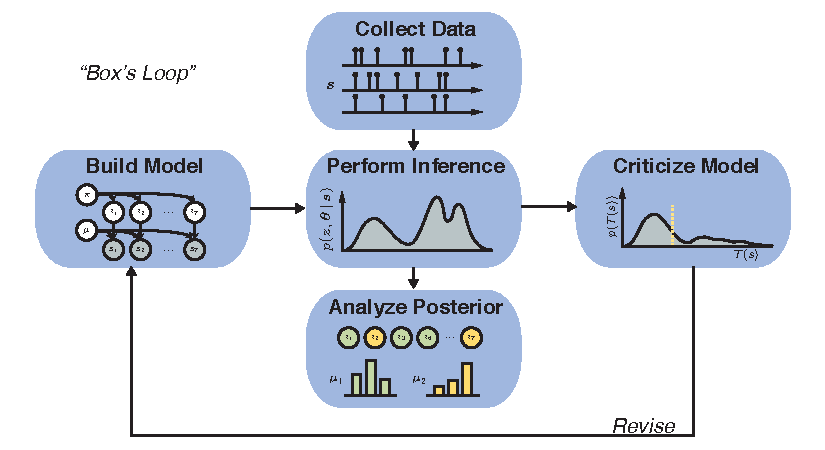
\includegraphics[width=5.5in]{figures/ch1/boxloop} 
\caption[Box's Loop]{Box's loop for hypothesis driven probabilistic modeling.
Adapted from~\citet{blei2014build}.}
\label{fig:boxloop}
\end{figure}


Figure~\ref{fig:boxloop} shows how crafting a probabilistic model and
performing Bayesian inference fit, conceptually, within the iterative
process of scientific study. \citet{blei2014build}, from whom this
figure has been adapted, calls this ``Box's loop'' in deference to the
foundational work of \citet{box1980sampling}. Each iteration is an 
experiment, and each experiment begins with a hypotbhesis, in the 
form of a model, and a computation, in the form of Bayesian inference.
Inferred posterior distributions over variables and parameters may 
lead to new insights about the data via exploratory analyses, and 
they may lead to further refinements of the theory via model criticism.


% Compositionality, scientific method and iterative experimental design
% exploratory analysis: summarize, visualize, hypothesize

% Model criticism, active learning, revision

% Not the first...
% cf Sahani 1999

\TODO{We are certainly not the first to advocate a Bayesian approach...
  but previous approaches were stifled by the challenges inherent in performing
  Bayesian inference in sophisticated models. We extend previous
  work by developing a host of new models that combine structured
  prior distributions, motivated by theoretical models of neural
  computation, with dynamic models of neural spike trains. We develop
  corresponding inference algorithms that enable efficient Bayesian
  inference in these hierarchical models.}


\section{Summary of Contributions}

\paragraph{Chapter 1} First we provide the necessary background on point processes and probabilistic modeling.

\paragraph{Chapters 2 and 3}

\paragraph{Chapter 4}

\paragraph{Chapter 5}

\paragraph{Chapter 6}

\paragraph{Chapter 7}
